\section[Lower bound under concentration assumption]{Lower Bound for Private Online learning under Concentration assumption}
\label{sec:main}

In this section, we provide the main result of our work along with their proof. Before stating the main result in~\Cref{thm:main-finite}, we need to define the concept of~\emph{distinguishing tuple} and \(\conc{\beta}\) learners.



\begin{definition}\label{defn:dist-tuple}
    Given \(f_0, f_1 \in \hyp\) and \(\xeq, \xdif \in \cX\), we call the tuple \((f_0, f_1, \xeq, \xdif)\) \emph{distinguishing},
    if  it satisfies both \(f_0(\xeq) = f_1(\xeq)\) and \(f_0(\xeq) = f_0(\xdif) \neq f_1(\xdif)\).
\end{definition}
A distinguishing tuple means that there are two functions (\(f_0, f_1\)), and two input points (\(\xeq, \xdif\)), such that only one of these points can effectively differentiate between the two functions. 
The absence of a distinguishing tuple implies a restricted hypothesis class: either \(\mathcal{H}\) is a singleton (\(\Card{\hyp} = 1\)), or it contains precisely two inversely related functions (\(\Card{\hyp} = 2\) with \(f_1 = 1 - f_0\)). In the latter case, \emph{every} input point contains information distinguishing \(f_1\) and \(f_2\).
This implies that there is no difference between input sequences, and the mistake bound will not depend on \(T\). For the purposes of our analysis, we proceed under the assumption that a distinguishing tuple always exists.


Let \((f_0, f_1, \xeq, \xdif)\) be a distinguishing tuple and suppose that adversary chooses \(f^{\ast} \in \Set{f_0, f_1}\).
Knowing only information on \(f^{\ast}(\xeq)\) does not help to tell apart \(f_0\) from \(f_1\).
Furthermore, if an algorithm is `too confident', meaning that it strongly prefers output of \(f_0\) on \(\xdif\) over output of \(f_1\), 
it will necessarily make a mistake on \(\xdif\) if \(f^{\ast} = f_1\). We will use this basic intuition to obtain our main lower bound and we will call such learners `concentrated', as defined below.

For input \(\tau\), index \(t \in [T]\) and an input point \(x \in \cX\), 
we denote \(\cA(\tau)_t \bs{x}\) to be the value of the \(t\)-th output function of \(\cA(\tau)\) evaluated at point \(x\).
\begin{definition}\label{defn:beta-conc}  
    An algorithm \(\alg\) is called \(\conc{\beta}\), 
    if there exists a distinguishing tuple \((f_0, f_1, \xeq, \xdif)\), such that
    \begin{equation}
        \Pr \bs{\forall t \in [T],\ \alg \br{\tau_0}_t\bs{\xdif} = f_0(\xdif)} \geq 1 - \beta,
    \end{equation}
    where \(\tau_0 = \br{\br{\xeq, f_0(\xeq)}, \ldots, \br{\xeq, f_0(\xeq)}}\).
\end{definition}
Note that \(\tau_0\) from~\Cref{defn:beta-conc} is a `dummy', \emph{non-distinguishing} input, as it does not contain any information to distinguish \(f_0\) from \(f_1\).

\subsection{Main Result}\label{sec:finite_horizon_result}
We now show that if the learner is both differentially private and concentrated, it will necessarily suffer a large (logarithmic in \(T\)) number of mistakes  in the game of~\Cref{def:general}.
\begin{theorem}\label{thm:main-finite}
Let \(\hyp\) be an arbitrary hypothesis class. Let \(\e > 0\), \(\delta \leq \e^2\) and \(T \leq \exp(1 / (32\delta))\).
If, for some \(\delta \leq \beta \leq 1/10\), \(\alg\) is a \(\beta\)-concentrated \((\e, \delta)\)-\Gls{dp} online learner of \(\hyp\), then there exists an adversary \(\cB\), such that
    \begin{equation}
        \E \bs{\regret_{\alg}} = \widetilde\Omega\br{\frac{\log T / \beta}{\e}},
    \end{equation}
    where \(\widetilde \Omega\) contains logarithmic in \(\e\) factors. For \(T > \exp(1 / (32\delta))\), \(\E \bs{\regret_{\alg}} = \widetilde\Omega\br{1/\delta}\).
\end{theorem}

 Before comparing our lower bound with known upper bounds, we first discuss the condition \(T\leq \exp(1 / (32\delta))\). Our bound suggests that for sufficiently large \(T\), specifically when \(T\) exceeds \(\exp(1 / (32\delta))\), the dependency on \(T\) is in fact not needed.
This can be seen from the following simple \emph{Name \& Shame} algorithm:  initialize an empty set \(S\); at each step, apply~\Gls{soa} and output \(\mathrm{\Gls{soa}}(S)\); upon receiving a new entry \((x_t, f^\ast(x_t))\), add it to \(S\) with probability \(\delta\). Clearly, this algorithm is \((0, \delta)\)-\Gls{dp}, since for any fixed input point, it only depends on this point with probability \(\delta\).
Furthermore, each time the algorithm incurs a mistake, it adds this mistake to \(S\) with probability \(\delta\). Since the algorithm runs \Gls{soa} on \(S\), it will make on expectation at most \(\ldim{\hyp} / \delta\) mistakes.
This algorithm is, however, not `conventionally' private, since it potentially discloses a \(\delta\)-fraction of the data, namely the set \(S\).

Now, we compare result of~\Cref{thm:main-finite} with known upper bounds in~\Cref{fig:lower-bound}. Recall that~\Gls{dpsoa} in \citet{golowich2021littlestone} obtained an upper bound which increases logarithmically with the time horizon \(T\).~\Cref{fig:lower-bound} shows that for \(T \leq \exp(1 / (32\delta))\), the dependency on \(T\) is necessary, thereby showing the tightness of~\Gls{dpsoa}~\citep{golowich2021littlestone}. For  larger \(T\), the aforementioned \emph{Name \& Shame} actually outperforms~\Gls{dpsoa}, indicating that, for fixed \(\e, \delta\), \emph{online algorithm always compromises privacy at very large \(T\)}. However, even for smaller \(T\), the plot shows that the number of mistake must grow with increasing \(T\) until it matches the \emph{Name \& Shame} algorithm.

\begin{figure}[t]\centering\vspace{-20pt}
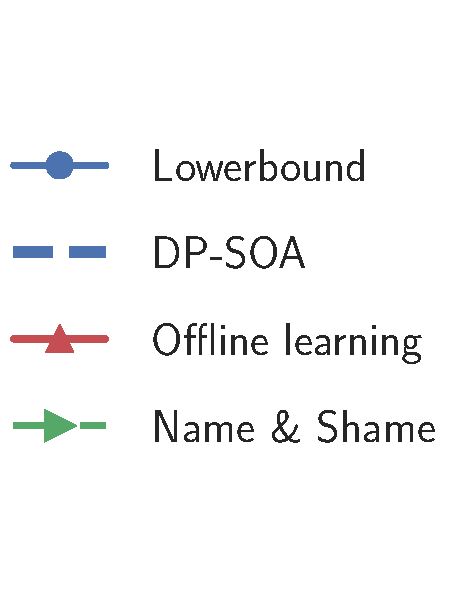
\includegraphics[width=0.2\linewidth]{chapters/dp/content/figures/legend.pdf}\quad\quad
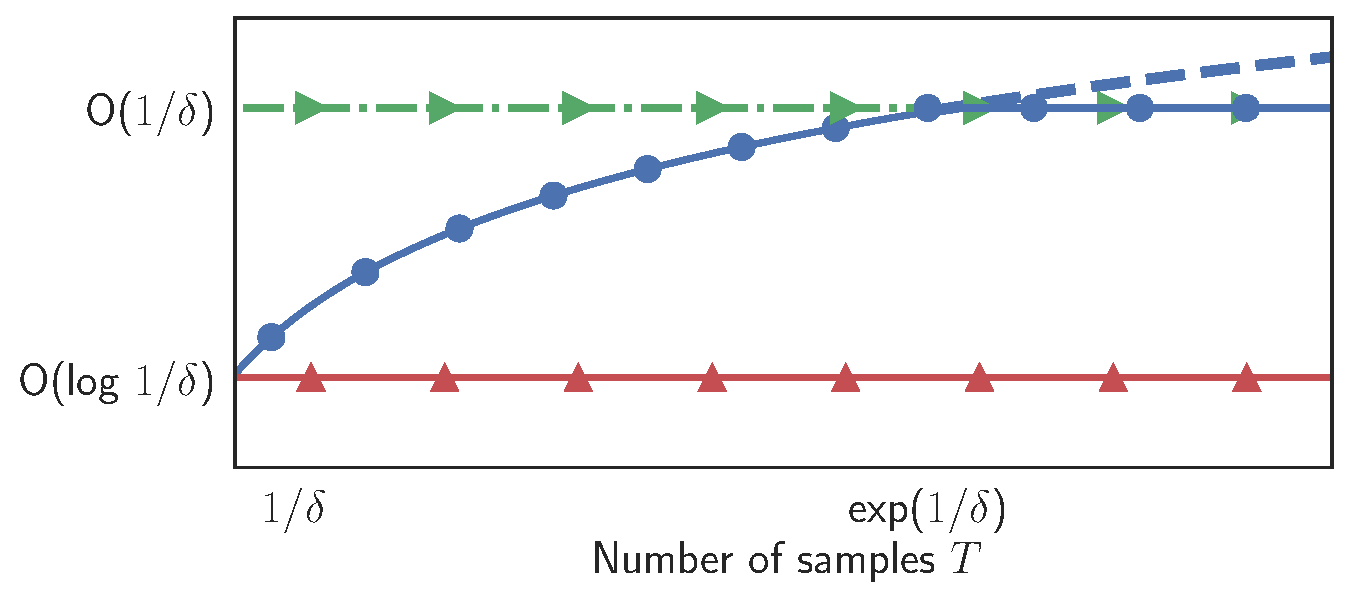
\includegraphics[width=0.6\linewidth]{chapters/dp/content/figures/lb_comp_markers_no_leg.pdf}
\caption{\small Lower bound from~\Cref{thm:main-finite} vs. existing upper bounds. We assume that \(\eps, \delta\) are fixed and for simplicity ignore dependence on \(\eps\). X-axis corresponds to the number of samples, growing from \(T \sim 1/\delta\) to \(T \sim \exp(1/\delta)\) and larger. Y-axis shows the expected number of mistakes, \(\E \bs{M_{\alg}}\).\vspace{-15pt}}
\label{fig:lower-bound}
\end{figure}

The main idea behind the construction of the lower bound is the following: assume that there is a distinguishing tuple \((f_0, f_1, \xeq, \xdif)\), such that \(\alg\) on \((\xeq, \ldots, \xeq)\) with high probability only outputs functions that are equal to \(f_0\) at \(\xdif\). Then, the adversary picks \(f^* = f_1\) and its goal is to select time steps \(t\) to insert \(\xdif\), such that (i) \(\alg\) with high probability will make a mistake at \(t\), and (ii) \(\alg\) will not be able to `extract a lot of information' from this mistake. As we show, both of these conditions can be guaranteed using the~\Gls{dp} property and concentration assumption of \(\alg\).
Note that if adversary inserts \(\xdif\) serially starting from \(t = 1\), \(\alg\) can have regret much smaller than \(\log T\). For example, if \(\alg\) first incurs a constant number of mistakes, the group privacy property allows a considerable change in the output distribution to only output \(f_1 = f^*\). But this is possible only if \(\alg\) can predict in advance, where it will make the mistake in the future.

Therefore, the adversary needs to `disperse' the points \(\xdif\) across \(T\) time steps, such that \(\alg\) cannot predict, where it might make the next mistake. We begin our construction by first inserting a point at the beginning. Then, depending on whether the leaner anticipates more points \(\xdif\) in the first half \emph{or} in the second half of the sequence, we insert \(\xdif\) in the half where it least expects it. Note that because of the concentration and~\Gls{dp} assumption, the learner cannot anticipate points \(\xdif\) in both halves simultaneously (recall that on input sequence consisting of only \(\xeq\), learner does not output a correct function for \(\xdif\)). By continuing this construction recursively, we are able to insert \(\Omega(\log T)\) points \(\xdif\), such that with constant probability, on each of them \(\alg\) will make a mistake.


\begin{proof}[of~\Cref{thm:main-finite}]
    Since \(\alg\) is \(\conc{0.1}\), there exists a distinguishing tuple \(\br{f_0, f_1, \xeq, \xdif}\), such that 
    \begin{equation}
        \Pr \bs{\forall t \in [T],\ \alg \br{\tau_0}_t\bs{\xdif} = f_0(\xdif)} \geq 0.9,
    \end{equation}
    where \(\tau_0 = \br{\br{\xeq, f_0(\xeq)}, \ldots, \br{\xeq, f_0(\xeq)}}\).
    WLOG assume that \(f_0(\xeq) = f_0(\xdif) = 0\).
    When \(T > \exp(1 / (32\delta))\), by simply only using the first \(\exp(1 / (32\delta))\) rounds, we obtain the required lower bound \(\widetilde\Omega(1 / \delta)\). In the remaining, we assume that \(T \leq \exp(1 / (32\delta))\).
    Furthermore, let \(k\) be the largest integer, such that \(2^k - 1 \leq T\). 
    Note that \(\frac{1}{2}\log{T} \leq k \leq 2\log T \leq 1/(16\delta)\). 
    For simplicity, we also assume that \(T = 2^k - 1\). We start with the case \(\e = \e_0 = \log\br{3/2}\) and pick \(f^\ast = f_1\) for the adversary.
    
    Note that to show \(\E \bs{M_\alg} = \Omega\br{\log T / \beta}\), we can construct two adversaries, first achieving~\(\E \bs{M_\alg} = \Omega\br{\log 1 / \beta}\)~(\textbf{Case I}) and the other~\(\E \bs{M_\alg} = \Omega\br{\log T}\)~(\textbf{Case II}). We now prove each of them.\\~\
    
    \noindent\textbf{Case I:}~We start with showing the adversary for the former bound, i.e., such that \(\E \bs{M_\alg} = \Omega\br{\log 1 / \beta}\).
    The concentration assumption implies that for any \(t \in [T]\), \(\Pr\br{\alg\br{\tau_0}_t\bs{\xdif} = 1} \leq \beta\).
    Therefore, if \(\tau_k\) contains \(k\) copies of the point \((\xdif, 1)\),  by applying~\Gls{dp} property of \(\alg\) \(k\) times, we obtain that for any \(t \in [T]\),
    \(\Pr\br{\alg\br{\tau_k}_t\bs{\xdif} = 1} \leq \beta \exp(k \e_0) + \delta \br{\frac{\exp\br{k\e_0} - 1}{\exp(\e_0) - 1}} \leq (k \delta + \beta)\exp(k \e_0)\).
    If \(k = \frac{1}{8 \e_0} \log (1 / \beta)\), we derive that for any \(t \in [T]\), 
    \begin{equation}
    \begin{aligned}
        \Pr(\alg(\tau_k)_t\bs{\xdif} = 1) &\leq (k \delta + \beta) \exp(k \e_0) \\
        &\leq \frac{\delta \log (1/\delta)}{8 \delta^{1/8} \e_0} \leq \frac{1}{3} \delta^{1/2} \log (1 / \delta) \leq \frac{1}{2}.
    \end{aligned}
    \end{equation} This implies that for the sequence \(\tau_k\), expected number of mistakes is \(\E\bs{M_{\alg}} \geq \frac{1}{16 \e_0} \log (1 / \beta)\). 
    
    \noindent\textbf{Case II:} In the previous case, it did not matter where exactly the points \((\xdif, 1)\) are inserted. However, if we want to prove the lower bound \(\Omega(\log T)\), this is no longer true and one needs to be careful with the placement of the inserted points.

    In the following, we construct a sequence \(\inpseq = \br{x_1, \ldots, x_T}\), such that expected number of mistakes of \(\alg\) will be large. We proceed iteratively, maintaining scalar sequences \((l_i), (r_i)\), and sequences \(\inpseq^{(i)}\) such that 
    \begin{enumerate}
        \item \(\inpseq^{(i)}\) contains exactly \(i\) points \(\xdif\) on the prefix \([1, l_i - 1]\),
        \item \(p_i \coloneqq \Pr\bs{\forall t \in [1, l_i - 1],\ \alg(\inpseq^{(i)})_t\bs{\xdif} = 0} \geq 1/2 - 4i\delta\),
        \item \(
          q_i \coloneqq \Pr\bs{
            \begin{aligned}
              &\forall t \in [1, l_i - 1],\ \alg(\inpseq^{(i)})_t\bs{\xdif} = 0 \textbf{ and } \\
              &\exists t \in [l_i, r_i],\ \text{ s.t. } \alg(\inpseq^{(i)})_t\bs{\xdif} = 1
            \end{aligned}
          } \leq 2\delta.
        \)
      \end{enumerate}
    Assume that we obtain these sequences until \(i = k \geq \frac{1}{2} \log T\). Then on the event \(\Set{\forall t \in [1, l_k - 1], \alg(\inpseq^{(i)})_t\bs{\xdif} = 0}\), \(\alg\) will make \(k\) mistakes. Since \(k \leq 1/(16\delta)\), from the second property above \(p_k \geq 1/4\). This implies that for the sequence \(\inpseq^{(k)}\) we have \(\E\bs{\regret_{\alg}} \geq p_k k \geq \frac{1}{8} \log T\).
    
     We construct the sequences by induction, starting with \(\inpseq^{(0)} = \br{\xeq, \ldots, \xeq}\). 
     For each \(i\), \(\inpseq^{(i)}\) will differ from \(\inpseq^{(i+1)}\) at exactly one point. 
     This allows us to use \Gls{dp} property of \(\alg\) in order to compare outputs on \(\inpseq^{(i)}\) and \(\inpseq^{(i+1)}\). 
     From \(\conc{0.1}\) assumption, we can pick \(l_0 = 1, r_0 = T\) which gives \(p_0 = 1\) and \(q_0 = 0.1\) (we interpret \(\Pr\bs{\forall t \in \emptyset \ldots} = 1\)).

    Given \(\inpseq^{(i)}\) we construct \(\inpseq^{(i+1)}\) by substituting \(l_i\)-th input point with \(\xdif
    \):
    \begin{enumerate}
        \item Let \((\inpseq^{(i+1)})_j = (\inpseq^{(i)})_j\) for all \(j \neq l_i\),
        \item Set \((\inpseq^{(i+1)})_{l_i} = \xdif\).
    \end{enumerate}
    Now we compute \(l_{i+1}, r_{i+1}\) and bound \(p_{i+1}, q_{i+1}\). To do this, we first introduce
    \begin{equation}
        \begin{aligned}
            &p'_i \coloneqq \Pr\bs{\forall t \in [1, l_i],\ \alg(\inpseq^{(i)})_t\bs{\xdif} = 0} \geq p_i - q_i, \\
            &q'_i \coloneqq \Pr\bs{
                \begin{aligned}
                    &\forall t \in [1, l_i],\ \alg(\inpseq^{(i)})_t\bs{\xdif} = 0\ \textbf{ and } \\
                    &\exists t \in [l_i + 1, r_i],\ \text{ s.t. } \alg(\inpseq^{(i)})_t\bs{\xdif} = 1
                \end{aligned}
            } \leq q_i,
        \end{aligned}
        \end{equation}
    which just account for the shift \(l_i \to l_i+1\). 
    Note that, since the events are nested, we can compute \(p'_i - q'_i = \Pr\bs{\forall t \in [1, r_i], \alg(\inpseq^{(i)})_t\bs{\xdif} = 0} = p_i - q_i\).
    Next, for \(m_i = (l_i + r_i) / 2\) and for any \(\bm{x} \in \Set{\xeq, \xdif}^T\), define
    \begin{equation}
        \begin{aligned}
            Q(\bm{x}) &\coloneqq \Set{
                \begin{aligned}
                    &\forall t \in [1, l_i],\ \alg(\bm{x})_t\bs{\xdif} = 0\ \textbf{ and } \\
                    &\exists t \in [l_i + 1, r_i],\ \text{ s.t. } \alg(\bm{x})_t\bs{\xdif} = 1
                \end{aligned}
            }, \\
            Q_1(\bm{x}) &\coloneqq \Set{
                \begin{aligned}
                    &\forall t \in [1, l_i],\ \alg(\bm{x})_t\bs{\xdif} = 0\ \textbf{ and } \\
                    &\exists t \in [l_i + 1, m_i],\ \text{ s.t. } \alg(\bm{x})_t\bs{\xdif} = 1
                \end{aligned}
            }, \\
            Q_2(\bm{x}) &\coloneqq \Set{
                \begin{aligned}
                    &\forall t \in [1, m_i],\ \alg(\bm{x})_t\bs{\xdif} = 0\ \textbf{ and } \\
                    &\exists t \in [m_i + 1, r_i],\ \text{ s.t. } \alg(\bm{x})_t\bs{\xdif} = 1
                \end{aligned}
            }.
        \end{aligned}
        \end{equation}
    Clearly, for any \(\bm{x}\), \(Q(\bm{x}) = Q_1(\bm{x}) \cup Q_2(\bm{x})\) with \(Q_1(\bm{x}) \cap Q_2(\bm{x}) = \emptyset\).
    Therefore,
    \begin{equation}
    \begin{aligned}
        q'_i = \Pr\bs{Q(\inpseq^{(i)})} = \Pr\bs{Q_1(\inpseq^{(i)})} + \Pr\bs{Q_2(\inpseq^{(i)})}.
    \end{aligned}
    \end{equation}
    We can use DP property of \(\alg\) when comparing outputs on \(\inpseq^{(i)}\) and \(\inpseq^{(i+1)}\) to get
    \begin{equation}\label{eq:q-i-plus-one}
    \begin{aligned}
    &\min\br{\Pr\bs{Q_1(\inpseq^{(i+1)})}, \Pr\bs{Q_2(\inpseq^{(i+1)})}}\\
    &\quad\leq \frac{1}{2} (\Pr\bs{Q_1(\inpseq^{(i+1)})} + \Pr\bs{Q_2(\inpseq^{(i+1)})})\\ 
    &\quad= \frac{1}{2} \Pr\bs{Q(\inpseq^{(i+1)})} \\
    &\quad\leq \frac{1}{2} \br{\exp(\varepsilon_0) \Pr\bs{Q(\inpseq^{(i)})} + \delta} \\
    &\quad= \exp(\varepsilon_0)q'_i /2 + \delta/2 \leq \frac{3}{4}q_i + \delta/2.
    \end{aligned}
    \end{equation}
    If \(\Pr\br{Q_1(\inpseq^{(i+1)})} \leq \Pr\br{Q_2(\inpseq^{(i+1)})}\) we set \(l_{i+1} \coloneqq l_i + 1, r_{i+1} \coloneqq m_i\), which gives \(q_{i+1} = \Pr\br{Q_1(\inpseq^{(i+1)})}\) and \(p_{i+1} = p'_i \geq p_i - q_i\) . 
    When \(\Pr\br{Q_1(\inpseq^{(i+1)})} > \Pr\br{Q_2(\inpseq^{(i+1)})}\), we set \(l_{i+1} = m_i + 1, r_{i+1} = r_i\), with \(q_{i+1} = \Pr\br{Q_2(\inpseq^{(i+1)})}\). We can bound 
    \begin{equation}
        \begin{aligned}
            p_{i+1} &= \Pr\br{\forall t \in [1, m_i],\ \alg(\inpseq^{(i+1)})_t\bs{\xdif} = 0} \\
            &= \Pr\br{\forall t \in [1, l_i],\ \alg(\inpseq^{(i+1)})_t\bs{\xdif} = 0} \\
            &\quad - \Pr\br{
                \begin{aligned}
                    &\forall t \in [1, l_i],\ \alg(\inpseq^{(i+1)})_t\bs{\xdif} = 0\ \textbf{ and } \\
                    &\exists t \in [l_i + 1, m_i],\ \text{ s.t. } \alg(\inpseq^{(i+1)})_t\bs{\xdif} = 1
                \end{aligned}
            } \\
            &= p'_i - \Pr\br{
                \begin{aligned}
                    &\forall t \in [1, l_i],\ \alg(\inpseq^{(i+1)})_t\bs{\xdif} = 0\ \textbf{ and } \\
                    &\exists t \in [l_i + 1, m_i],\ \text{ s.t. } \alg(\inpseq^{(i+1)})_t\bs{\xdif} = 1
                \end{aligned}
            } \\
            &\geq p'_i - \frac{3}{2} \Pr\br{
                \begin{aligned}
                    &\forall t \in [1, l_i],\ \alg(\inpseq^{(i)})_t\bs{\xdif} = 0\ \textbf{ and } \\
                    &\exists t \in [l_i + 1, m_i],\ \text{ s.t. } \alg(\inpseq^{(i)})_t\bs{\xdif} = 1
                \end{aligned}
            } \\
            &= p'_i - \frac{3}{2} q'_i = p_i - q_i - \tfrac{1}{2} q'_i \geq p_i - \tfrac{3}{2} q_i,
        \end{aligned}
        \end{equation}
    where we used the DP property for the first inequality.
    % , and the fact that \(p_i - q_i = \Pr\br{\forall t \in [1, r_i], \alg(\inpseq^{(i)})_t\bs{\xdif} = 0} = p'_i - q'_i\).
    % Otherwise, we set \(l_{i+1} = m_i + 1, r_{i+1} = r_i\), with \(q_{i+1} = \Pr\br{Q_2(\inpseq^{(i+1)})}\) and 
    % \(p_{i+1} \geq p'_i - q'_i \geq p_i - 2q_i\). 
    Overall, we obtain with our choice of \(l_{i+1}, r_{i+1}\):
    \begin{equation}
    \label{eq:q-i-p-i-recursion}
    q_{i+1} \leq \frac{3}{4} q_i + \delta / 2 \quad \text{and} \quad p_{i+1} \geq p_i - 2q_i.    
    \end{equation}
    By geometric sum properties, we have that \(q_i \leq \frac{1}{10} (3/4)^i + 2\delta\), and therefore, \(p_i \geq 1/2 - 4i \delta\).
    Finally, note that \(r_{i+1} - l_{i+1} = (r_i - l_i) / 2 - 1\). In the beginning we have \(r_0 - l_0 = 2^k - 2\), therefore \(r_i - l_i = 2^{k - i} - 2\). Thus, we can repeat this process \(\frac{1}{2} \log T \leq k \leq 2 \log T \leq 1/(16\delta)\) times. By construction, all inserted points \(\xdif\) for \(\inpseq^{(i)}\) lie on the prefix \([1, l_i - 1]\). In order to extend to other values of \(\e\), we either insert more points per step (if \(\e < \e_0\)), 
    or divide the segment into more parts (if \(\e > \e_0\)). We refer to~\Cref{app:all-eps} for the argument in these cases. This concludes the proof.
\end{proof}

\subsection{Examples of \(\conc{\beta}\) online learners for \(\point_N\)}
\label{sec:example-conc}
Next, we show that several learners that could be used for online learning \(\point_N\), satisfy~\Cref{defn:beta-conc}. In particular, in~\Cref{lem:example-conc-learners} we prove that any improper learner that learns \(\point_N\) using a finite union of hypothesis in \(\point_N\)~(defined as Multi-point in~\Cref{defn:multi-point}) is concentrated. \Cref{lem:dpsoa-conc} implies that the only existing private online learning algorithm~\Gls{dpsoa} is concentrated.


\begin{definition}[Multi-Point class]\label{defn:multi-point}
     For \(1 \leq K \leq N \in \N_+\), we define \(
        \point^K_N\)
    to be the class of functions that are equal to 1 on at most \(K\) points.
\end{definition}
\begin{lemma}\label{lem:example-conc-learners}
    Let \(\beta > 0\) and \(K, T \in \N_+\). 
    For any \(N \geq 3K T^2 / \beta\), any learner \(\alg\) of \(\point_N\) that only uses \(\point^K_N\) as its output set is \(\conc{\beta}\).
\end{lemma}
\begin{proof}
    Set \(\xeq = 1\) and \(f_1 = \bI\bc{ \cdot = 2}\).
    Let \(\tau_0 = \br{\br{\xeq, f_1(\xeq)}, \ldots, \br{\xeq, f_1\br{\xeq}}}\) and
    \(\alg(\tau_0) = (\hat f_1, \ldots, \hat f_T)\).
    For \(t \in [T]\), let \(
        Q_t = \Set{x \in [N], \text{ such that } \Pr\br{\hat f_t(x) = 1} \geq \beta / T}\).
    We can write
    \begin{equation}
    \begin{aligned}
        &\sum_{x \in [N]} \Pr(\hat f_t(x) = 1) = \sum_{x \in [N]} \sum_{\substack{f \in \point^K_N \\ f(x) = 1}} \Pr(\hat f_t = f)
        \\
        &\quad = \sum_{f \in \point^K_N} \sum_{\substack{x \in [N] \\ f(x) = 1}} \Pr(\hat f_t = f) \leq K \sum_{f \in \point^K_N} \Pr(\hat f_t = f) = K,
    \end{aligned}
    \end{equation}
    which implies that \(\Card{Q_t} \leq K \lceil T / \beta \rceil\).
    Therefore, by union bound, as long as \(N \geq 3K T^2 / \beta\), there exists \(\xdif \in \left([N] \setminus \bigcup_{t=1}^T Q_t\right) \setminus \Set{1, 2}\).
    Applying union bound again, we obtain that 
    \begin{equation}
        \Pr(\exists t, \text{ such that } \hat f_t(\xdif) = 1) \leq \sum_{t=1}^T \Pr(\hat f_t(\xdif) = 1) \leq \beta.
    \end{equation}
    Thus, \(\alg\) is \(\conc{\beta}\) and the distinguishing tuple is \((f_1, \bI\bc{ \cdot = \xdif}, \xeq, \xdif)\).
\end{proof}

In~\Cref{lem:example-conc-learners} we assumed that \(K\) is a constant. Note that as long as \(K = o(N)\), by taking \(N\) large enough one can obtain the same result. We also remark that the~\Gls{soa} for \(\point_N\), which is an improper learner, uses \(\point_N^1\) as the output hypothesis class.~\citet{beimel2014bounds} also uses improper learners consisting of union of points for privately learning \(\point_N\) in the pure \Gls{dp}-\Gls{pac} model; their hypothesis class is a subset of the Multi-Point class.\footnote{ See Section 4.1 in~\citet{beimel2014bounds} to see the conditions that the hypothesis class needs to satisfy.} 

While their motivation was to explicitly construct a smaller hypothesis class that~\emph{approximates} \(\point_N\) well, on a more general note, it is also common to use larger hypothesis classes in computational learning theory for improper learning. This is particularly useful for benefits like computational efficiency~(e.g.,~3-DNF vs 3-CNF) and robustness~\citep{diakonikolas2019distribution}. The purpose of~\Cref{lem:example-conc-learners} is to show that natural improper learners using larger hypothesis classes for \(\point_N\), like~\Cref{defn:multi-point}, are also \(\mathrm{concentrated}\). Furthermore, as we show next, the only generic private online learner that we are aware of---~\Gls{dpsoa}, is also concentrated.
\begin{corollary}\label{lem:dpsoa-conc}
    \(\dpsoa\) for \(\point_N\) is \(\conc{\beta}\) for any \(N \geq 3 T^2 / \beta\).
\end{corollary}
\begin{proof}
    Output of \(\dpsoa\) is equal to the output of \(\soa\) algorithm on some input sequence. 
    Note that \(\soa\) for \(\point_N\) is always equal to either (i) an all-zero function, or (ii) a target function \(f^{\ast}\),
    which implies that it lies in \(\point^1_N\).
    Therefore, by~\Cref{lem:example-conc-learners}, we obtain that \(\dpsoa\) is also \(\conc{\beta}\).
\end{proof}


\noindent\textbf{Independent work} In a concurrent and independent work,~\citet{cohen2024lower} established that learners that \emph{are not} concentrated must nevertheless suffer large expected regret for the specific case of \(\point_T\). They construct an adversary which strongly relies on the large size of the function class. In particular, generalizing for a smaller function classes, e.g.~\(\point_3\) remains an interesting open question. We obtain a partial progress in this direction, see~\Cref{sec:beyond_conc}.

